% !TeX root = skripta-konstitutivni-vztahy-materialu.tex
% !TeX lastmodified = 2019-12-11

\subsection{Použití viskoplastických modelů}
Pokud plastická deformace významně závisí na rychlosti zatěžování, jedná se o chování viskoplastické (viz obr. \ref{fig:zavislost-mezni-plochy-plasticity}).

Viskoplastické modely umožňují popsat mezní plochy plasticity pro široké rozmezí rychlostí zatěžování,
od nekonečně malých (rovnovážný stav) po velmi vysoké (rázové děje).
U~kovů jsou potřebné, pokud absolutní teplota překročí $\frac{1}{4}$ teploty tavení kovu. 

\begin{figure}
	\label{fig:zavislost-mezni-plochy-plasticity}
	\centering
	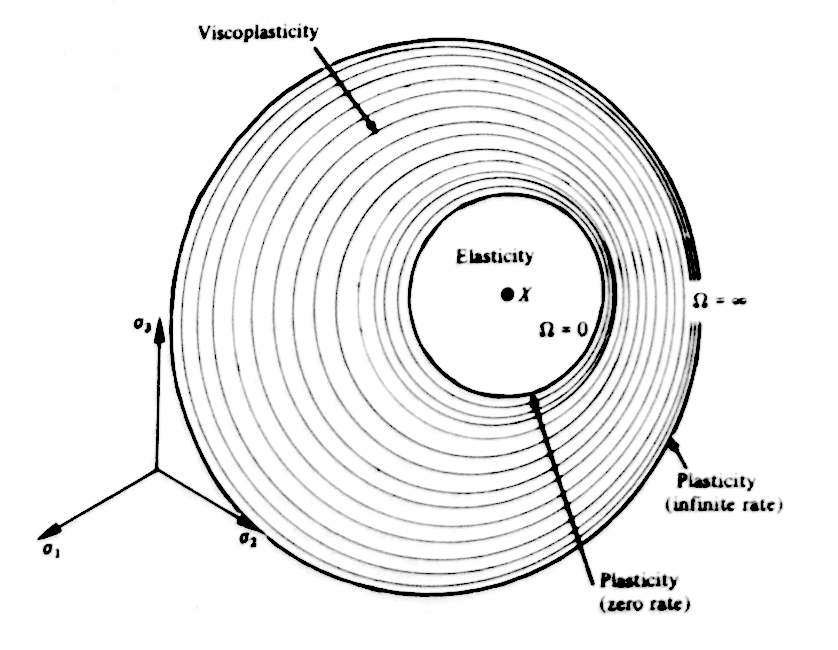
\includegraphics[width=0.7\linewidth]{zavislost-mezni-plochy-plasticity}
	\caption{Závislost mezní plochy plasticity na rychlosti zatěžování}
\end{figure}

\subsubsection{Model (visko)plasticity Johnson-Cook}\label{sec:johnson-cook-viskoplasticita}
Tento viskoplastický model\footnote{Johnson G. R., Cook W. H. Fracture characteristics of three metals subjected to various strains, strain rates, temperatures and pressures. Engineering Fracture Mechanics, 1985, vol. 21, pp. 31-48.} zohledňuje vliv rychlosti deformace a~teploty na plastické chování materiálu a~je navíc schopen popsat také porušení.
Jeho křivka zpevnění je dána rovnicí pro redukované (Misesovo) napětí
\begin{equation}
	\bar{\sigma} = \left[ \sigma_y + K (\bar{\varepsilon}_p)^n \right] \left[ 1 + C \ln(\dot{\varepsilon}^*) \right] \left[ 1 - (T^*)^m \right],
\end{equation}
kde
\begin{description}
	\item[$\bar{\varepsilon}_p$] je redukované plastické přetvoření,  
	\item[$\dot{\varepsilon}^* = \tfrac{\dot{\bar{\varepsilon}}_p}{\dot{\bar{\varepsilon}}_0}$] je bezrozměrná rychlost redukovaného plastického přetvoření,
	\item[$\dot{\bar{\varepsilon}}_p$] je rychlost redukovaného plastického přetvoření,
	\item[$\dot{\bar{\varepsilon}}_0$] je referenční rychlost přetvoření, obvykle při standardní tahové zkoušce (měla by být kvazistatická),
	\item[$T^* = \tfrac{T-T_0}{T_m-T_0}$] se nazývá homologická teplota, kde 
	$T$, $T_m$, $T_0$ značí aktuální teplotu, teplotu tavení a~pokojovou teplotu $[\si{\kelvin}]$.
	\item[$\sigma_y$] je mez kluzu,
	\item[{$K\:[\si{\mega\pascal}], n\:[-]<1, C\:[-], m\:[-]$}] jsou další parametry modelu.
\end{description}

\subsubsection{Materiálové zkoušky pro viskoplastický model}
Pro identifikaci modelu je třeba experimentálně určit závislost na rychlosti zatěžování a~na teplotě; jsou nutné minimálně následující zkoušky:
\begin{itemize}
	\item Kvazistatická zkouška za pokojové teploty\\
	Při ní je $\dot{\bar{\varepsilon}} = 1$ a~$T^* = 0$, takže fitujeme jen koeficienty v první závorce ($K$, $n$).
	\item Kvazistatická zkouška za zvýšené teploty\\
	Pokud proběhne při stejné rychlosti deformace, můžeme exponent 	teplotního změkčení určit ze vztahu
	\begin{equation}
		m = \frac{\log(1-R)}{\log(T^*_1)},
	\end{equation}
	kde
	\begin{equation*}
		R = \frac{1-(T^*_1)^m}{1-(T^*_2)^m}
	\end{equation*}
	\item Dynamická zkouška za pokojové teploty\\
	Z této zkoušky se určí konstanta $C$ (pro $T^* = 0$) pro bezrozměrnou rychlost redukovaného plastického přetvoření určenou z~obou zkoušek jako
	\begin{equation}
		\dot{\varepsilon}^* = \frac{\dot{\bar{\varepsilon}}_p}{\dot{\bar{\varepsilon}}_0}
	\end{equation}
\end{itemize}

\begin{figure}
	\label{fig:vliv-zvyseni-teploty-johnsoon-cook}
	\centering
%	\includegraphics[width=0.5\linewidth]{}
	\caption{Vliv zvýšení teploty o~\SI{200}{\kelvin} na deformačně-napěťovou křivku}
\end{figure}
	